\section{Dynamic Delay Scheduling}\label{sec:dynamic}

\subsection{Beyond Constant Delays}

The frameworks described above use a fixed delay interval, 
which remains the same throughout an entire job. Our observation is that there is a 
calculable tipping point after which waiting/skipping is no longer beneficial. Generally,
we can define the total running time of a task \textit{t} as:

\[
t\_total = t\_compute + t\_netOH + sch\_delay
\]

where \textit{t\_compute} is the local computation time of the task, \textit{t\_netOH}
is the network latency incurred from data transfer (this is zero if the task is scheduled 
locally), and \textit{sch\_delay} is the amount of time \textit{t} is delayed 
(skipped) to wait for locality, from the moment \textit{t} is first considered for 
scheduling.

Ideally, we want to minimize the task completion time of all tasks within a given job, 
while also providing some guarantee as to the maximum latency introduced by the scheduler
itself through delay scheduling. The goal of delay scheduling is to remove \textit{t\_netOH} by 
scheduling a task locally, but if the task is delayed longer than the delay interval, 
then it would have actually been more efficient in hindsight (in terms of task completion time) 
to immediately schedule the task in the first open slot that was considered. 
Conversely, if the delay interval is too short, then the task could potentially miss 
scheduling opportunities with locality, which would result in a shorter completion time
than scheduling without locality.

Dynamic Delay Scheduling improves upon fixed delay scheduling by dynamically adapting the maximum 
\textit{sch\_delay} equal to \textit{t\_netOH} on a per-task basis. This allows 
for the longest waiting time for data-local slots while limiting the worst case task 
running time to \textit{t\_compute + (2 * t\_netOH)}. In this way, the delay interval
will adapt to the severity of the network overhead. If \textit{t\_netOH} is low, then locality
is less of a concern and the scheduler can shorten the time it delays. If \textit{t\_netOH} becomes high,
then the scheduler increases the time that it waits, as locality is more important in poorer network
conditions; however, this means that the 
network overhead incurred by running tasks needs to be monitored and reported to the 
scheduler over time, in order to adapt to changing network conditions and potentially 
heterogeneous data block sizes. To calculate the network overheads (i.e., one-way trip delay + data transferring time), we can use the ping utility to calculate one-way trip (i.e., round-trip time / 2) while available bandwidth between source and destination nodes over the network can be calculated with available bandwidth measurement tools, which will be further discussed in the following Section.

%What else can affect on:
%Preemption
%Scheduler policies (fairness or more locality)

\subsection{Available Bandwidth in Datacenter Environments}\label{sec:band}


\begin{figure}[t]
	\minipage{0.5\textwidth}
		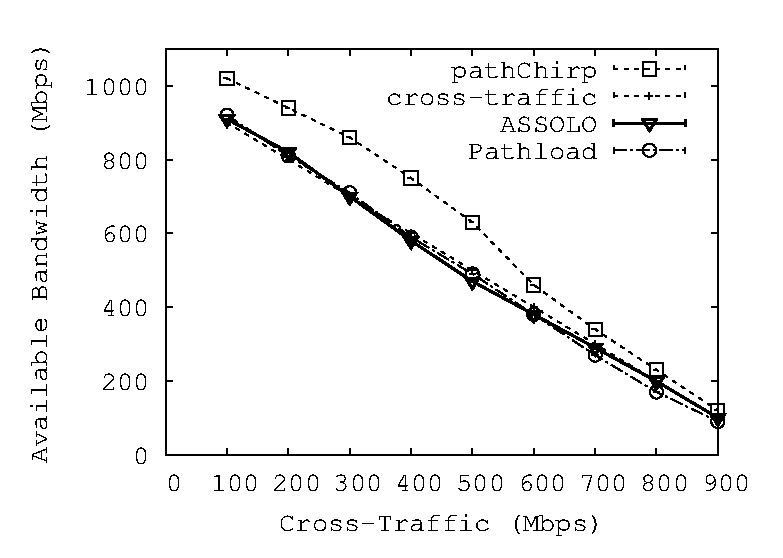
\includegraphics[width=\linewidth]{./figures/avail-bw.eps}
		\caption{avail-bw as a function of offered cross-traffic load}
		\label{fig:avail-bw}
	\endminipage \hfill
\end{figure}

The available bandwidth (avail-bw) in a network path is of major importance in
congestion control, streaming applications, QoS verification, server selection,
and overlay networks. Several tools (i.e., Pathload, yaz, spruce, abing, dietTopp,
ASSOLO, Abing, IGI, pathChirp, PTR, and etc.) have been introduced and verified
on the Internet~\cite{Goldoni:2010}. However, avail-bw measurements in datacenter environments have not been performed yet.
Considering network condition differences between the Internet and datacenters,
network topology in datacenters has relatively simpler and lesser hops in
end-to-end paths. Among the available avail-bw measurment tools, we tested
pathload~\cite{ Jain:2003}, ASSOLO~\cite{Goldoni:2009}, and pathChrip~\cite{Ribeiro:2005}
 based on their accuracy and intrusiveness.
 We use D-ITG~\cite{Botta:2012} as a traffic generator and vary cross traffic load from 100 Mbps
  and 900 Mbps in 1Gbps end-to-end path capacity. We measure each tool on
  how much avail-bw varies based on offered loads. To avoid edge effects, we started
 measurement tools several seconds later after starting cross-traffic and reported each measurement over a 300 second duration.
 As shown in Figure~\ref{fig:avail-bw}, we have confirmed that Pathload and ASSOLO
 provided similar behavior and quite high fidelity, while pathChrip consistently overestimates
 available bandwidth by more than 10\%, which is a well-known issue and also reported in~\cite{Goldoni:2010, Shriram:2005}.

Intrusiveness is another important metric of avail-bw measurement tools, as it causes a significant decrease in the avail-bw and increases delays or losses. This can be measured by how much probe traffic has been injected during the measurement. As reported in ~\cite{Goldoni:2010}, ASSOLO and pathChrip inject probe traffic lesser than 0.3 Mbits/sec, while Pathload injects probe traffic more than 30 Mbits/sec. Compared to Pathload and pathChrip, ASSOLO provides better tradeoffs between accuracy and intrusiveness. Thus, we adopt ASSOLO as our network available bandwidth measurement tool.  A recent 19 months measurement study regarding a wide variety of applications on Amazon EC2 has reported that EC2 provides stead network conditions such as bandwidth and latency to provide reliable performance to support bandwidth-intensive and latency-sensitive applications~\cite{Hajjat:2015}.


% It has also reported that traffic in datacenter has steady network condition on EC2 ("Application-speific configuration selection in the cloud by Hajjat et al"


%Throughly analyze all O/Hs caused by choosing machine in the same rack and a different rack (RRT/2, NIC data rate (i.e, Tx and Rx), E2E available bandwidth, additional operation (i.e., serialization and deserialization, and etc.)

%Stable bandwidth in Amazon EC2 ~\cite{Hajjat:2015}


\subsection{An Adaptive Solution Using Task Feedback}

The network overhead incurred by missing data locality depends on many factors, including 
network traffic, the distance of a task from its data, and the input data size. These 
factors vary from job to job, and some (like network traffic) can change during the job 
execution itself. In order to adapt the delay scheduling interval to changing conditions, 
we have designed a simple feedback mechanism, in which each task reports the network overhead it experienced 
upon completion (\textit{t\_netOH}, for a task \textit{t}). This metric is sent to a 
centralized fair scheduler, which then changes its delay scheduling interval using a 
running average of feedback from completed tasks. This new delay scheduling interval is 
then used when scheduling subsequent tasks of the same type.

The feedback metric itself (\textit{t\_netOH}) can be any time measurement which 
reflects the network overhead incurred by a task. In the case of Dynamic Delay Scheduling, we are 
considering tasks which read data from distributed file systems,
so the \textit{t\_netOH} for each task is the amount of time spent 
reading data blocks remotely; however, any arbitrary type of task, which has some way of 
measuring its own overhead, could set this as well and benefit from the adaptation.

%\newcommand{algrule}[1][.2pt]{\par\vskip.5\baselineskip\hrule height #1\par\vskip.5\baselineskip}

\begin{algorithm}[]
    \footnotesize
    \DontPrintSemicolon
    \caption{Dynamic Delay Scheduling}
    \textbf{Initialization:}\;
    delay\_interval $\leftarrow$ default (3 seconds)\;
    \hrule width 0.4\textwidth
    \;
    \textbf{Upon receiving task $t$ completion event:}\;
    delay\_interval $\leftarrow$ (delay\_interval + t.netOH) / 2\;
    \hrule width 0.4\textwidth
    \;
    \textbf{Scheduling Procedure:}\;
    \For{each open slot $s$ on a node $n$ in N}{
        sort $J$ in increasing order of currently running tasks\;
    
        \For{$j$ in $J$}{
            \If{$j$ has just launched a task}{
                $j$.wait\_begin = current\_time\;
            }
            \eIf{a task $t$ in $j$ has data on $s$'s node $n$}{
                launch t in $s$\;
            }{
                \If{a task $t$ in $j$ is unlaunched}{
                    \eIf {current\_time - $j$.wait\_begin $>$ delay\_interval}{
                        launch $t$ in slot $s$\;
                    }{
                        continue\;
                    }
                }
            }
        }
    }
\end{algorithm}


Algorithm 1 describes our adaptive solution in detail, in a cluster with \textit{N} nodes and \textit{J} jobs. 
When tasks complete, the delay interval will be changed to reflect 
recent overhead measurements. The delay interval adapts relatively quickly (the average of
the last few readings), since feedback can only be received when tasks complete. For workloads
in which tasks complete very often, the window for the average can be broadened. 
During scheduling, this new interval is used for delay scheduling (and this interval can 
change even while a job is currently waiting, as tasks complete). It is worth noting that 
there is nothing preventing this adaptive solution from also being hierarchical, as many 
frameworks desire/implement separate delay intervals for node-local or rack-local scheduling.

